\documentclass[8pt,xcolor=table,aspectratio=169]{beamer}

\usepackage{graphicx}
\usepackage{caption}
\usepackage{subcaption}
\usepackage{transparent}
\usepackage{epstopdf} %converting to PDF
\usepackage{multicol} 
\usepackage{animate}[2017/05/18]

\usepackage{amsmath}
\usepackage{amssymb}
\usepackage{mathtools}
% \usepackage[utf8]{inputenc}
% \usepackage[T1]{fontenc}
% \usepackage[thinc]{esdiff}

% \usepackage{pdfx}
 
% \usepackage[utf8]{inputenc}
% \usepackage[T1]{fontenc}
\usepackage[table]{xcolor}    % loads also »colortbl« 
%  \usepackage{enumitem}
% \usepackage{ucltemplate}
\usepackage{color}

\usepackage{comment}

\usepackage{tabularx} % make width of table columns evenly distributed (see http://tex.stackexchange.com/questions/60601/evenly-distributing-column-widths)
% \newcolumntype{Y}{>{\centering\arraybackslash}X}

% make entire row bold or italic in table
\newcommand\setrow[1]{\gdef\rowmac{#1}#1\ignorespaces}
\newcommand\clearrow{\global\let\rowmac\relax}
\clearrow


\usepackage{amssymb}% http://ctan.org/pkg/amssymb
\usepackage{pifont}% http://ctan.org/pkg/pifont
\newcommand{\cmark}{\ding{51}}%
\newcommand{\xmark}{\ding{55}}%


%\usepackage{pgfgantt} % for grantt charts
\usepackage{rotating}
\usepackage[graphicx]{realboxes}
\usepackage[export]{adjustbox}
\usepackage{array}

\usepackage{rotating}
% \usepackage{tabularx, booktabs} % make width of table columns evenly distributed (see http://tex.stackexchange.com/questions/60601/evenly-distributing-column-widths)
% \newcolumntype{Y}{>{\centering\arraybackslash}X}

\DeclareMathOperator*{\argmin}{arg\,min}
\DeclareMathOperator*{\argmax}{arg\,max}

\usepackage{tikz}
\usetikzlibrary{bayesnet}
\usetikzlibrary{decorations}
\usetikzlibrary{decorations.pathreplacing}
\usetikzlibrary{arrows,positioning, shapes.symbols,shapes.callouts,patterns,shapes,chains,calc,backgrounds,fadings}

% \definecolor{parCol}{rgb}{0.1, 0.1, 1}
% \definecolor{stCol}{rgb}{0.1, 0.6, 0.1}
% \definecolor{bothCol}{rgb}{0, 0.5, 0.5}

\definecolor{parCol}{rgb}{0, 0, 0}
\definecolor{stCol}{rgb}{0, 0, 0}
\definecolor{bothCol}{rgb}{0, 0, 0}
\definecolor{blue3}{HTML}{86B7FC} % med blue
\definecolor{blue1}{HTML}{B5F1FF} % light blue
\definecolor{blue2}{HTML}{E0F9FF} % very light blue

\newcolumntype{C}[1]{>{\centering\let\newline\\\arraybackslash\hspace{0pt}}m{#1}}

\setlength{\tabcolsep}{0.2em}

 
 %% OVERVIEW OF WORK SO FAR %%
 
%Information to be included in the title page:
\title{Medical Image Generation and Analysis\\ using\\ Bayesian Generative Models}
\author[Raz]{
R\u{a}zvan V. Marinescu\vspace{1em}}

\institute{\small{Massachusetts Institute of Technology}

% \vspace{0em}
% \small{Centre for Medical Image Computing, University College London, UK}
}

\date{}

% logo of my university
\titlegraphic{
   \begin{figure}
%    \begin{subfigure}{0.32\textwidth}
%    \hspace{2em}
%    
\includegraphics[height=1.0cm]{ucl_logo}
%    \end{subfigure}
   \begin{subfigure}{0.32\textwidth}
   \centering
   
\includegraphics[height=1.0cm]{MIT_logo.png} 
   \end{subfigure}
%    \begin{subfigure}{0.32\textwidth}
%    \centering
%    
\includegraphics[height=1.0cm]{pondLogo.png} 
%    \end{subfigure}
   \end{figure}
   
%    \tiny{Slides available online: https://people.csail.mit.edu/razvan/talk/martinos2019/pres.pdf}
}

\setbeamercolor{frametitle}{fg=black}
\setbeamercolor{author in head/foot}{fg=black, bg=white} 
\setbeamercolor{institute in head/foot}{fg=black, bg=white} 
\setbeamercolor{title in head/foot}{fg=black, bg=white}
\setbeamercolor{date in head/foot}{fg=black, bg=white}

\setbeamersize{text margin left=10pt,text margin right=10pt}
% \setbeamertemplate{frametitle}{
%     \vspace{0.9em}
%     \insertframetitle
% %     \vspace{-3em}
% }
\setbeamertemplate{frametitle}{%
    \vspace{0.5em}
    \usebeamerfont{frametitle}\insertframetitle%
    \vphantom{g}% To avoid fluctuations per frame
    %\hrule% Uncomment to see desired effect, without a full-width hrule
    \par% <-- added
    \hspace*{-\dimexpr0.5\paperwidth-0.5\textwidth}% <-- calculation of left margin width
    \rule[0.5\baselineskip]{\paperwidth}{0.4pt}%
}

\setbeamertemplate{footline}
{
  \vspace{-3em}
  \leavevmode%
   \rule{\paperwidth}{0.3pt}
  \hbox{%
  \begin{beamercolorbox}[wd=.2\paperwidth,ht=2.25ex,dp=1ex,center]{author in head/foot}%
    \usebeamerfont{author in head/foot}Razvan V. Marinescu
  \end{beamercolorbox}%
  \begin{beamercolorbox}[wd=.2\paperwidth,ht=2.25ex,dp=1ex,center]{institute in head/foot}%
    \usebeamerfont{institute in head/foot}razvan@csail.mit.edu
  \end{beamercolorbox}%
  \begin{beamercolorbox}[wd=.3\paperwidth,ht=2.25ex,dp=1ex,center]{institute in head/foot}%
    \usebeamerfont{institute in head/foot}http://razvan.csail.mit.edu
  \end{beamercolorbox}%
  \begin{beamercolorbox}[wd=.2\paperwidth,ht=2.25ex,dp=1ex,center]{title in head/foot}%
    \usebeamerfont{title in head/foot}\insertsection
  \end{beamercolorbox}%
  \begin{beamercolorbox}[wd=.10\paperwidth,ht=2.25ex,dp=1ex,right]{date in head/foot}%
    \usebeamerfont{date in head/foot}\insertshortdate{}\hspace*{2em}
    \insertframenumber{} / \inserttotalframenumber\hspace*{2ex}
  \end{beamercolorbox}}%
  \vskip0pt%
}

% \usepackage{beamerthemesplit}

\newcommand{\backupbegin}{
   \newcounter{finalframe}
   \setcounter{finalframe}{\value{framenumber}}
}
\newcommand{\backupend}{
   \setcounter{framenumber}{\value{finalframe}}
}


\makeatletter
\long\def\beamer@author[#1]#2{%
  \def\and{\tabularnewline}
  \def\insertauthor{\def\inst{\beamer@insttitle}\def\and{\tabularnewline}%
  \begin{tabular}{rl}#2\end{tabular}}%
  \def\beamer@shortauthor{#1}%
  \ifbeamer@autopdfinfo%
    \def\beamer@andstripped{}%
    \beamer@stripands#1 \and\relax
    {\let\inst=\@gobble\let\thanks=\@gobble\def\and{, }\hypersetup{pdfauthor={\beamer@andstripped}}}
  \fi%
}
\makeatother
\beamertemplatenavigationsymbolsempty
\setbeamertemplate{caption}[numbered]
\setbeamercolor{caption name}{fg=black}
\setbeamercolor{itemize item}{fg=black}
\setbeamercolor{itemize subitem}{fg=black}
\setbeamercolor{enumerate item}{fg=black}
\setbeamercolor{enumerate subitem}{fg=black}
\setbeamertemplate{enumerate item}[default]
\setbeamertemplate{enumerate subitem}[default]

\makeatletter
\let\@@magyar@captionfix\relax
\makeatother
\begin{document}
 
\section{Introduction}

\frame{\titlepage}
 
\setbeamerfont{frametitle}{size=\large}

\newcommand{\upgradeReportLoc}{../../upgrade_report}
\newcommand{\epsrcPresLoc}{\upgradeReportLoc/epsrcPres}
\newcommand{\jointModellingDiseaseLoc}{../../jointModellingDisease}
\newcommand{\pcaLongPaperLoc}{../../PCA_long_paper}
\newcommand{\voxFld}{../../voxelwiseDPM}
\newcommand{\tadpoleFld}{../../tadpole}
\newcommand{\diffEqModelFld}{../../diffEqModel}

\newcommand{\outFolder}{../overview/modelDiagram}
\newcommand{\lw}{0.5mm}

\newcommand{\yes}{{\LARGE \textcolor{green!50!black}{\checkmark} \par}}
\newcommand{\no}{{\LARGE \textcolor{red}{\xmark} \par}}



\definecolor{light-gray}{gray}{0.6}


\newcommand{\inc}[1]{\includegraphics[width=\columnwidth, trim=4 4 4 4, clip]{#1}}
\newcommand{\incw}[2]{\includegraphics[width=#2\columnwidth, trim=4 4 4 4, clip]{#1}}
\newcommand{\inch}[2]{\includegraphics[height=#2, trim=4 4 4 4, clip]{#1}}

\newcommand{\vo}{\vspace{1em}}
\newcommand{\vt}{\vspace{2em}}
\newcommand{\vth}{\vspace{3em}}



\begin{frame}{Long-term vision}

\vspace{-2em}
\begin{columns}[t]
\begin{column}{0.5\textwidth}
\centering

\textbf{\large Accurate diagnosis and prognosis through AI}\\
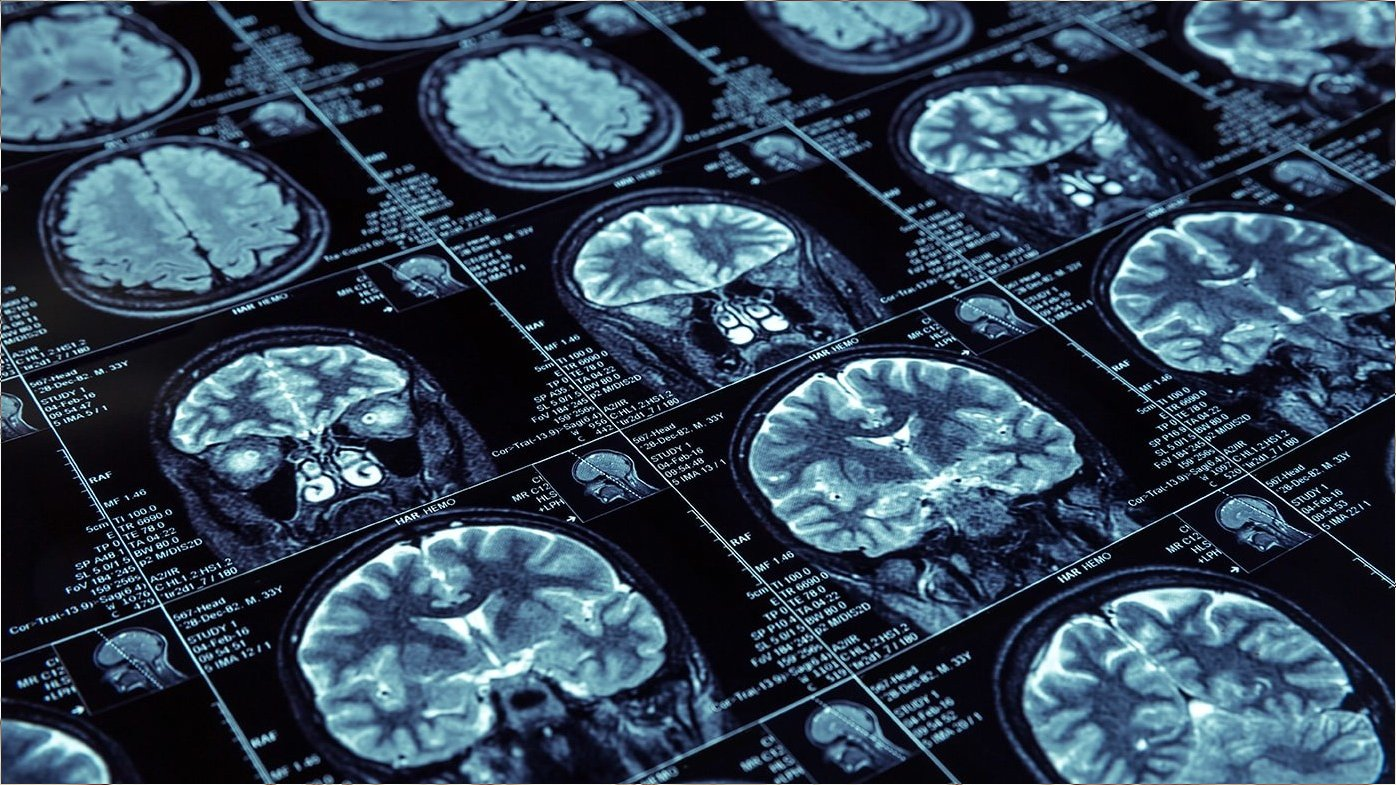
\includegraphics[height=4.3cm]{ai-diagnosis}


\end{column}
\begin{column}{0.5\textwidth}
\centering

\textbf{\large AI to augment humans}\\
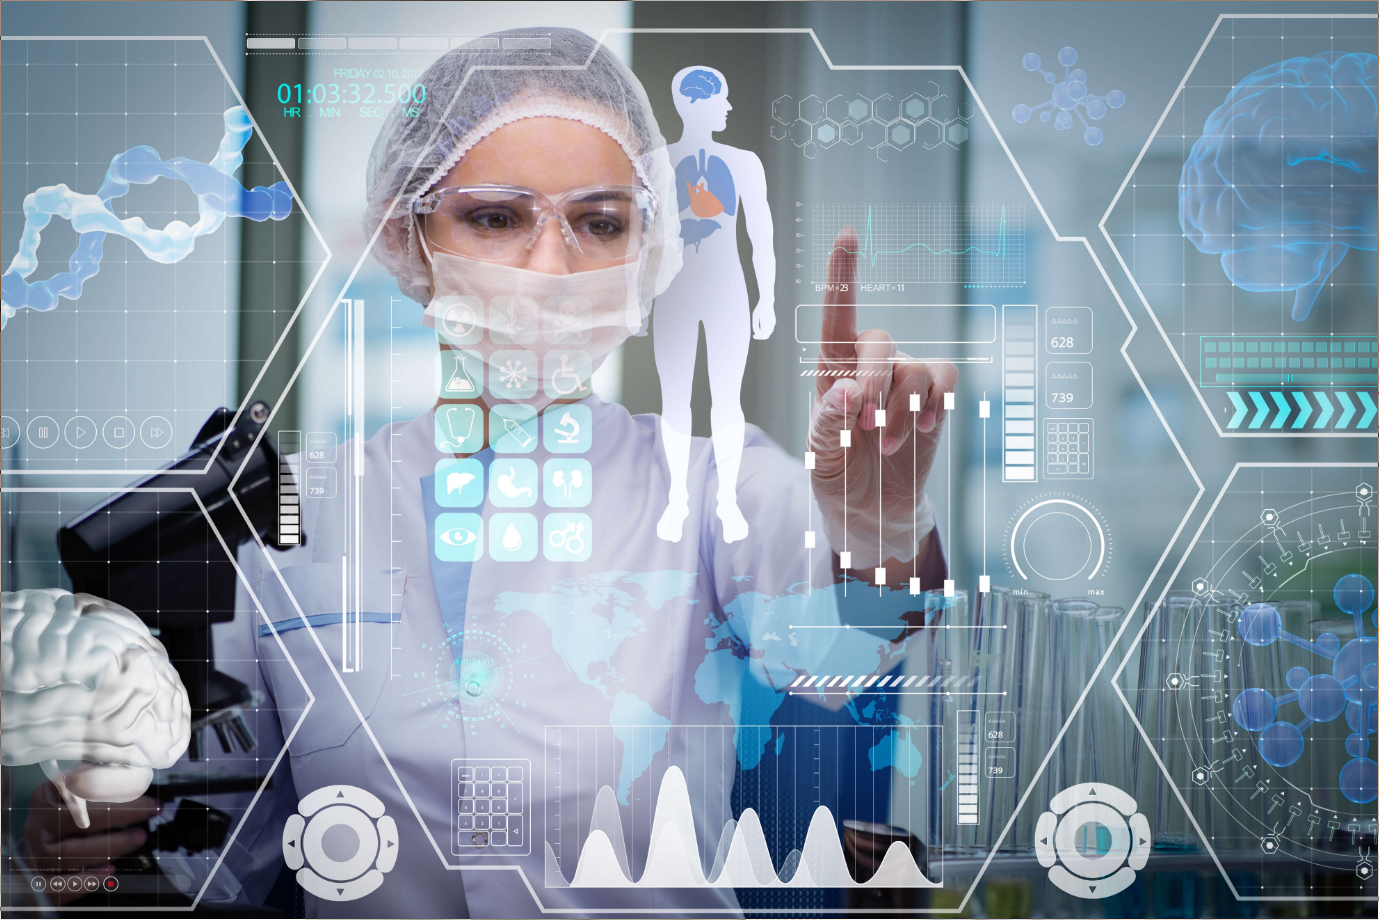
\includegraphics[height=4.3cm]{ai_augment_full}

\end{column}
\end{columns}

\end{frame}



\begin{frame}{Future work}


\vspace{-2em}
\begin{columns}
\begin{column}{0.5\textwidth}
\centering

Biological simulators\\
\incw{heartsim}{0.5}

\vt
\vt

Multimodal modelling\\
images + text + structural data  
\incw{xray}{0.3}\incw{medreport}{0.267}

\end{column}
\begin{column}{0.5\textwidth}
\centering

%Better and faster reconstruction of medical images\\
%\incw{mri_recon}{0.8}

%\vt
%\vt

Disease Progression Modelling
\incw{daninet}{1}

% \vo

% Domain knowledge from large-scale parsing of medical articles\\
% \incw{lotsoftext}{0.4}

\end{column}
\end{columns}


\end{frame}


\begin{frame}{Future work: Brain tissue and anatomy simulator}


Simulator for brain anatomy from genetics:
\begin{itemize}
 \item Using deep generative models
 \item Accounting for distributions shifts
 \item Following causal principles
\end{itemize}

\vt

\incw{brainsimulator}{0.9}

\end{frame}

%\begin{frame}{MRI reconstruction}
%
%\end{frame}


\begin{frame}{Multimodal modelling}

\begin{itemize}
\item Modalities: scan contrasts (T1/T2), Diffusion imaging, PET, diagnostic report
\onslide<3-> \item Later on, replace latent with genetics and covariates
\end{itemize}

\begin{columns}
\begin{column}{0.5\textwidth}
\centering
\onslide<2-> Generic latent space\\
\onslide<2-> \incw{future_multimodal}{0.5}
\end{column}
\begin{column}{0.5\textwidth}
\centering
\onslide<3-> Genetics as latent space\\
\onslide<3-> \incw{future_multimodal_part2}{0.5}
\end{column}
\end{columns}


\end{frame}

\begin{frame}{Disease Progression Modelling}

\begin{itemize}
\item Current models mostly work with features extracted from scans (low dimensionality)
\item Aim: make models work with raw, 3D scans
\item First  build a good 3D brain scan generator
\item Then estimate progression over time
\end{itemize}

\vo

\begin{columns}
\begin{column}{0.5\textwidth}
\centering
3D-StyleGAN
\incw{3dstylegan}{0.8}\\
(submitted to MICCAI, 2021)
\end{column}
\begin{column}{0.5\textwidth}
\centering
Disease Progression Modelling
\incw{daninet}{1}
\end{column}
\end{columns}

%\begin{center}
%
%\end{center}



\end{frame}

\end{document}



